\documentclass{article}
\usepackage[utf8]{inputenc}
\usepackage{graphicx}
\usepackage{epstopdf}
\usepackage{caption}
\usepackage{subcaption}
\usepackage{multirow}
\usepackage{hyperref}
\usepackage{url}
\usepackage{seqsplit}
\hypersetup{pdfstartview={FitH null null null}}
\usepackage{amssymb,amsmath}
\usepackage{amsthm}
\usepackage{empheq}
\usepackage{algorithm,algpseudocode}
\usepackage[margin=1.5in]{geometry}
\usepackage{listings}
\usepackage{program}
\usepackage{commath}
\lstset{language=Python} 

\usepackage{listings}
\usepackage{color} %red, green, blue, yellow, cyan, magenta, black, white
\definecolor{mygreen}{RGB}{28,172,0} % color values Red, Green, Blue
\definecolor{mylilas}{RGB}{170,55,241}


\title{Stochastic optimization of an objective function to build a 3D chromosomal model}
\author{Caiwei Wang, Xiaokai Qian, Sean Lander, \\Haipei Fan, Puneet Gaddam, Brett Koonce\\\\University of Missouri - Columbia}

\date{May 7, 2014}

\algloopdefx{NoEndIf}[1]{\textbf{If} #1 \textbf{then}}

\begin{document}

\maketitle

\begin{abstract}

First, we construct a congugate gradient (CG) descent searcher to build a 3D model of a human chromosome using the method advanced by Trieu and Cheng in a recent paper.  Next, we utilize two different stochastic methods, simulated annealing (SA) and Markov-Chain Monte-Carlo (MCMC), to duplicate our CG results.  Then, we build a PDB model of the final chromosome and visualize the process of solving the objective function.  Ultimately, we compare our results with other research in this domain, discuss difficulties we encountered and potential future improvements that could be made.

\end{abstract}

\section{Introduction}

The human genome has been sequenced, but modelling the human chromosome remains a difficult task.  One promising avenue of modern research lies in the technique of Hi-C sequencing, which produces contact maps as part of the sequencing process.  By analyzing which regions of the genome are often found together, we can build up a map of the larger genome.  Trieu and Cheng recently proposed a new method based on an objective function that promises to be able to build a model using gradient descent from the Hi-C data.  We decided to put their results to the test, as well as experiment with solving the objective function using stochastic (MCMC and SA) methods.

\section{Overview}

\begin{figure}[H]
\begin{center}
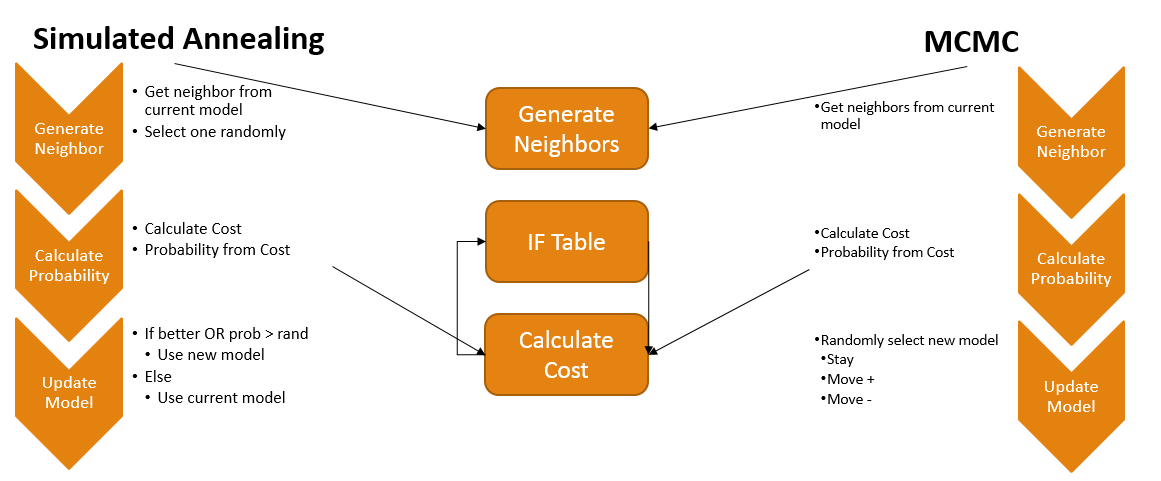
\includegraphics[width=\textwidth]{architecture}
\caption{Architecture Summary}
\label{Fig:architecture}
\end{center}
\end{figure}

We do not have a complicated pipeline for this project.  Essentially, we take input data, clean it up slightly, and apply one of three different methods: CG, SA, and MCMC.

\section{Dataset}

We obtained a megabase resolution fragment database (157x157, dropping first/last residues from Chromosome 7) from Trieu to work with.  We set all entries less than 0.66 to 0, as per the same treatment in the original paper.  We also made a list of the constants they used, so that our results would (hopefully) match.

\section{Objective function}

Simply put, the objective function advanced by Trieu and Cheng can be expressed as follows:

\begin{equation}
      TotalModelScore(m) = ContactScore(m) + NonContactScore(m) + PairSmoothing(m)
\end{equation}

The first operation minimizes the distances of contacts with affinity to keep them in contact (but keeps their distance above a minimum threshold):

\begin{equation}
      ContactScore(m) = \sum_{i=1}^{n} \sum_{j=1}^{n} (\abs{i-j}>1) * (W_1 * \tanh(d_c^2-d_{ij}^2) * N_{ij} + W_2 * \tanh(d_{ij}^2-d_{min}^2))
\end{equation}

The second operation maximizes the distances of contacts without affinity to keep them away from contact (but keeps their distance below a maximum threshold):

\begin{multline}
      NonContactScore(m) = \sum_{i=1}^{n} \sum_{j=1}^{n} (\abs{i-j}>1) * (W_3 * \tanh(d_{max}^2-d_{ij}^2) / TotalIF \\+ W_4 * \tanh(d_{ij}^2-d_{c}^2) / TotalIF)
\end{multline}

The third operation tweaks the scores of consecutive contacts slightly so that moving them is favored over adjusting more distant relationships:

\begin{multline}
      PairSmoothing(m) = \sum_{i=1}^{n} \sum_{j=1}^{n} (\abs{i-j}=1) * (W_1 * IF_{max} / TotalIF * \tanh(da_{max}^2-d_{ij}^2) \\+ W_2 * \tanh(d_{ij}^2-d_{min}^2) / TotalIF)
\end{multline}

We also used the following table of constants from Trieu and Cheng's paper.  They are experimentally derived values.

\begin{center}
\begin{tabular}{|l|c|c|c|r|}
\multicolumn{4}{c}{Constants} \\
    \hline
    $d_{min}$ & $\sqrt 0.2$ & W1 & 1.0           \\ \hline
    $d_{max}$ & 4.5  & W2 & 1.5      \\ \hline
    $d_{c}$ & $\sqrt 7.0$  & W3 & 1.5            \\ \hline
    $da_{max}$ & $\sqrt 1.8$  & W4 & 1.5     \\ \hline
    \end{tabular}
\end{center}

We also make use of the following:

\begin{equation}
      TotalIF = \sum_{i=1}^{n} \sum_{j=1}^{n} IF(i,j)
\end{equation}

\begin{equation}
      N(i,j) = IF(i,j)/TotalIF
\end{equation}

\begin{equation}
      IF_{max} = \max(IF(i,j),IF(j,i))
\end{equation}

Combining the above equations, we end up with a combined objective function of approximately 50000 subproblems, as detailed above.  Our problem now is simply to maximize the result given a 471 variable input vector (157 contacts * 3 coordinates $(x, y, z)$) across this space.  Towards this end, we present one deterministic and two stochastic methods of optimization.  For each version, our initial solution subspace is randomly chosen coordinates in the domain $-0.5 \leq (x, y, z) \leq 0.5$. 

\section{Conjugate Gradient Descent}

Our first method we applied is standard gradient descent.  We utilized a solver based upon the Powell conjugate method.  This allowed us to avoid calculating a derivative function.  Instead, it maintains a list of search vectors and attempts a bidirectional search along each one.  Each iteration, the highest performing vector is replaced by the best new search vector and then the process repeats.  This method is easy to implement, but takes some time to run.

\section{Simulated Annealing}

For our first test of stochastic methods, we built a simulated annealer capable of solving our objective function.  SA is a well known non-deterministic algorithm to sample a state space quickly.  Essentially, we start from a random model, then generate a neighboring model (our original model with a modification).  We score the two models.  If the new one is better, we accept it, otherwise we only replace our existing model based on a gradually decreasing schedule (temperature function).  As such, the two most important parts of implementing simulated annealing are the temperature function and how we generate neighbor models.

We tested the following two temperature functions, one sigmoid and one linear:

\begin{equation}
      T_s(e,t,k) =  -t*2/(1 + \exp(-5*k/t)) + t*2
    \end{equation}
\begin{equation}
      T_l(e,t,k) =  (-t/e)*k + t
    \end{equation}
    
For a neighborhood function, we select a contact at random.  Next, we generate a random offset, scaled using the known minimum contact distance: $d_{c}/2*(x,y,z)$.  Then, we score the two models using the method described previously.  For our simulated annealing schedule, we ended up using one million simulations (epochs) over a temperature range of 250 degrees.

\begin{figure}[H]
\begin{center}
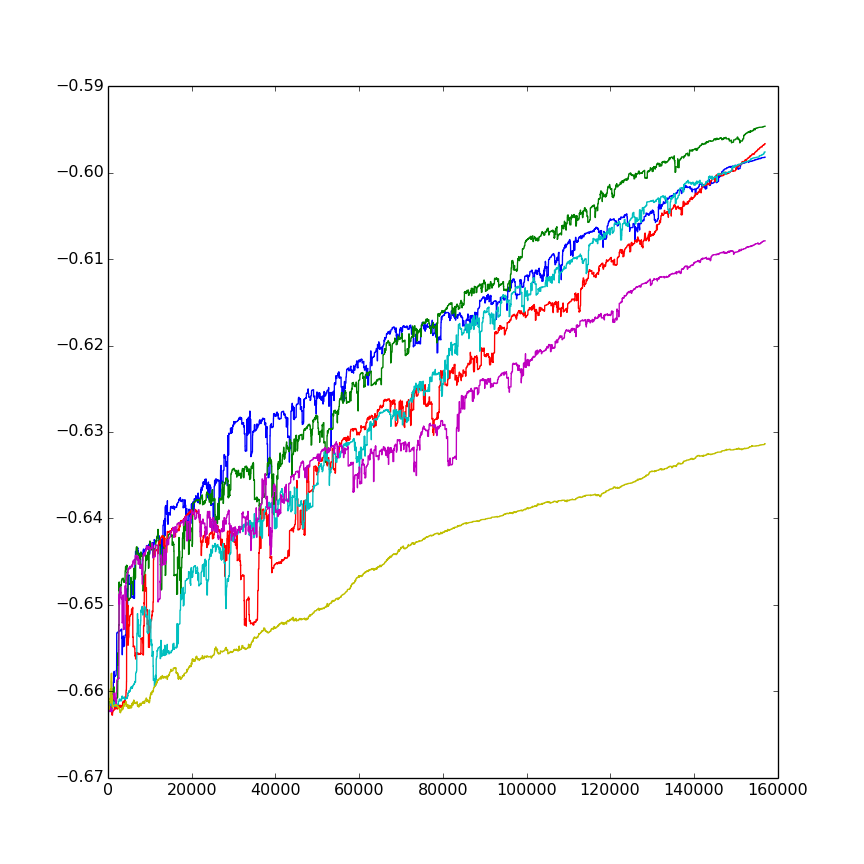
\includegraphics[width=\textwidth]{SA_Chromo7-Scores}
\caption{A graph of score versus number of simulations for SA: -n6-e157000-t250}
\label{Fig:sa_score_n6}
\end{center}
\end{figure}

\begin{figure}[H]
\begin{center}
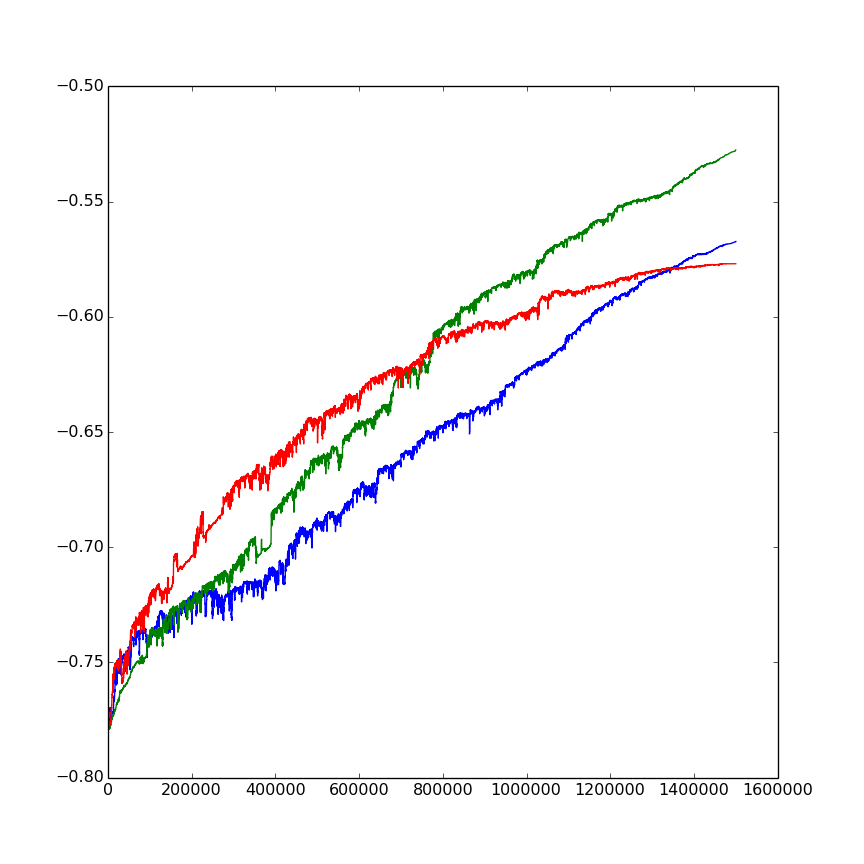
\includegraphics[width=\textwidth]{SA_None-Scores}
\caption{A graph of score versus number of simulations for SA: -n3-e1500000-t250}
\label{Fig:sa_score_none}
\end{center}
\end{figure}

\section{Markov-Chain Monte-Carlo}

For our second test of stochastic methods, we built a Markov-Chain Monte Carlo sampler.  Markov chains are an important technique in computer science from statistics.  First, we build up a graph model of discreet events with a corresponding transition matrix.  Next, we seed the transition matrix using real-world data (generally derived from posterior probability distributions).  Then, we can sample the Markov model repeatedly (Monte Carlo) to try and converge upon a solution space that is generally an excellent model of our problem domain.

For our project, we utilized MCMC to optimize our state/input vector (coordinate data) to most closely approximate our posteior distribution (our objective function).  Our methods converged well, but required a large number of simulations to mix (over one million simulations for the larger residues).  We utilized a different neighborhood function than we used in Simulated Annealing.  First, we select a random region from which to generate a neighborhood. The neighborhood is then created by increasing/decreasing the location in each of the three dimensions: $(x, y, z)$. In this way we generate 8 neighbors and a default position which are scored and given a probability of selection based on the score range, with higher scoring conformations more likely to be sampled. Once a new neighbor conformation is selected the process repeats until all iterations have completed.

We tested two different versions of MCMC: a greedy and non-greedy selector:

\begin{equation}
      T_{greedy} = (score - minScore) / scoreRange
    \end{equation}
\begin{equation}
      T_{non-greedy} = (score - minScore) / (scoreSum - minScore * neighborCount)
    \end{equation}

\begin{figure}[H]
\begin{center}
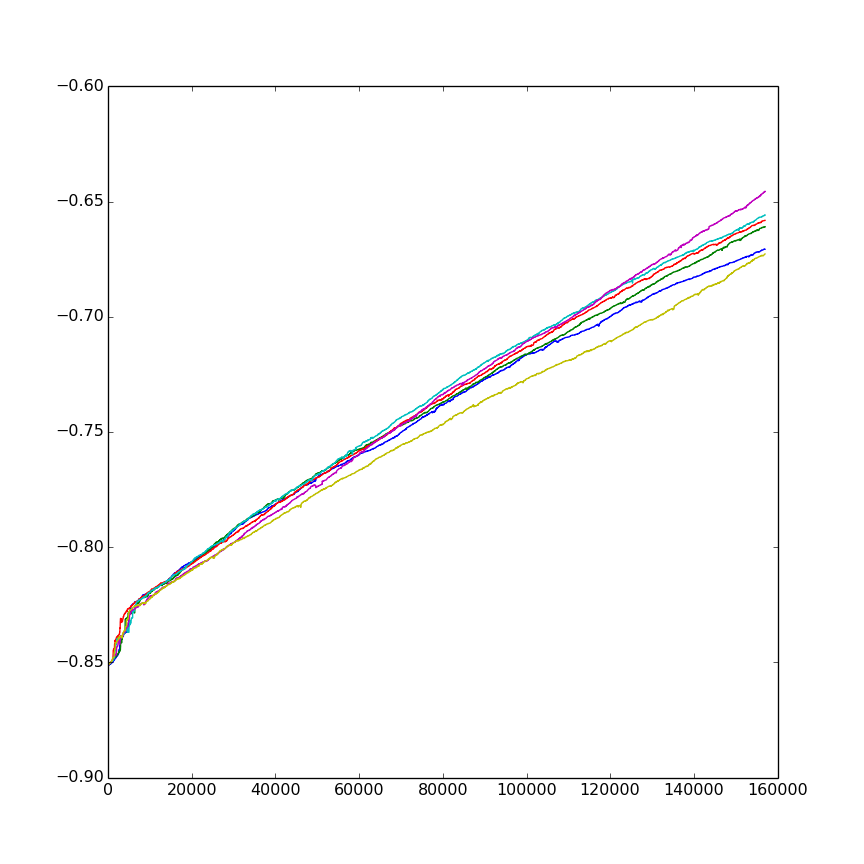
\includegraphics[width=\textwidth]{MCMC_Chromo7-Scores}
\caption{A graph of mixing versus number of simulations for MCMC: -n6-e157000}
\label{Fig:mcmc_mixing}
\end{center}
\end{figure}

\section{Results}

For testing purposes, we wrote tools to enable us to work on a subset of the final data (ten resiudes, for example).  This in turn allowed us to make sure that all of our methods converged to the same results and provided an objective benchmark.

Generally speaking, we found that:

\begin{enumerate}

\item Our conjugate gradient solver was not very fast, but provided accurate results.  Our usage of the Powell method, while easy to implement, was not very fair to this technique.  Since we know the objective function, we should have been able to build a derivative function by hand and in turn make this method much faster.

\item When utilizing an external solver, simulated annealing converged quickly and rapidly to a solution (approx. 5 minutes for a 157 residue chain).  Our custom SA solver was slower (approx. 600k-1.5 million simulations required).  We attribute this to that our neighborhood function did not change the state space very much and as a result the entire process required a lot more simulation time.  We ended up just using the linear temperature model and did not find that the sigmoid model offered much improvement.

\item We found that MCMC mixed (and found a solution) on our problem for smaller residue tests, but for the larger problem performance was too limited for us to recommend this technique going forward (we estimate \gt1 million simulations are needed for a full chain).  The table below is not entirely fair to MCMC, because our neighborhood function generates eight neighbors for each cycle.  In other words, the two methods are doing roughly the same amount of math, the problem is simply that MCMC does not converge as quickly as would be desired.\\

\end{enumerate}


\begin{center}
\begin{tabular}{|l|c|c|c|r|}
\multicolumn{2}{c}{Iterations/minute} \\
    \hline
    SA & 10,000 \\ \hline
    MCMC: greedy & 1750    \\ \hline
    MCMC: non-greedy & 1700    \\ \hline
    \end{tabular}
\end{center}

\section{Visualization}

To visualize our results (and get feedback on making sure our math was correct), we added a basic visualizer of the 3D line generated by the contact model.  Here is an example picture:


\begin{figure}[H]
\begin{center}
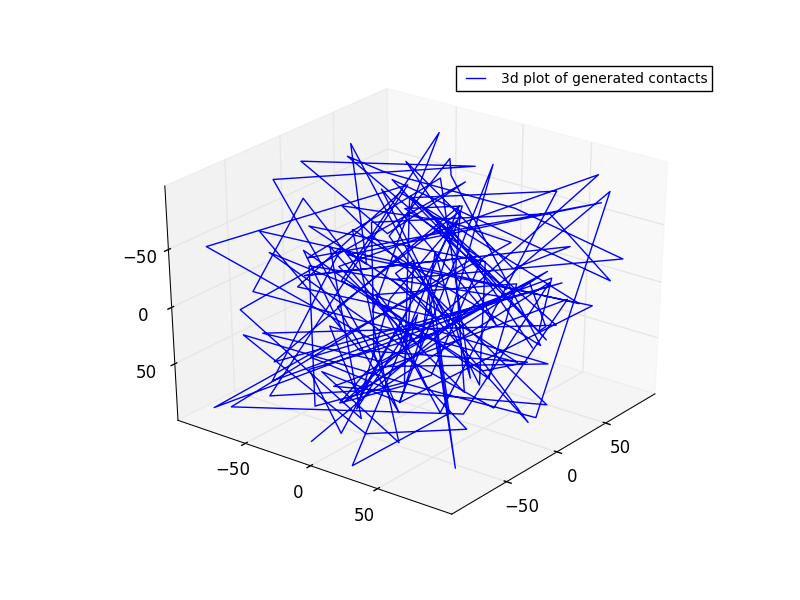
\includegraphics[width=\textwidth]{sa_150}
\caption{An visualization of the contact map generated by simulated annealing}
\label{Fig:sa_150}
\end{center}
\end{figure}

\section{Citations}

We thank the following tools and papers: \\

Tuan Trieu and Jianlin Cheng.  Large-scale reconstruction of 3D structures of human chromosomes from chromosomal contact data.  Nucl. Acids Res. first published online January 24, 2014. doi:10.1093/nar/gkt1411



\end{document}
